\chapter{Projet DN-Rider}
\label{chap:Projet DN-Rider}

\section{Constat \& Objectif du stage}


Objectif: une application web (IHM + API REST) pour manipuler les notes de livraison Katana:

\begin{itemize}
  \item gérer l'objet NDL de manière plus simple qu'avec nexus/filesystème
  \item éviter les tableaux de suivi, type notes d'installation / tableaux de dépendances / ..., édités manuellement
  \item fédérer certaines fonctionnalités (extraction d'information, identification des package a installer sur une plateforme...) par rapport aux scripts bash/groovy/perl/ruby....
  \item  outiller le suivi du cycle de vie des versions par rapports aux infos remontées par les outils de l'usine logicielle et Katana
\end{itemize}

L’application devra être légère, dynamique et facilement évolutive, et non-contraignante pour les équipes.

Le but est de fiabiliser le processus de livraison/mise en production des applications.
\clearpage

\section{Contexte \& Démarche}
\paragraph{Equipe Intégration / Accompagnement Projet (transverse)}
\paragraph{Travail autonomie / equipe}
\paragraph{Démarche agile ( kanban) (devops)}

\begin{figure}[h]
\centering
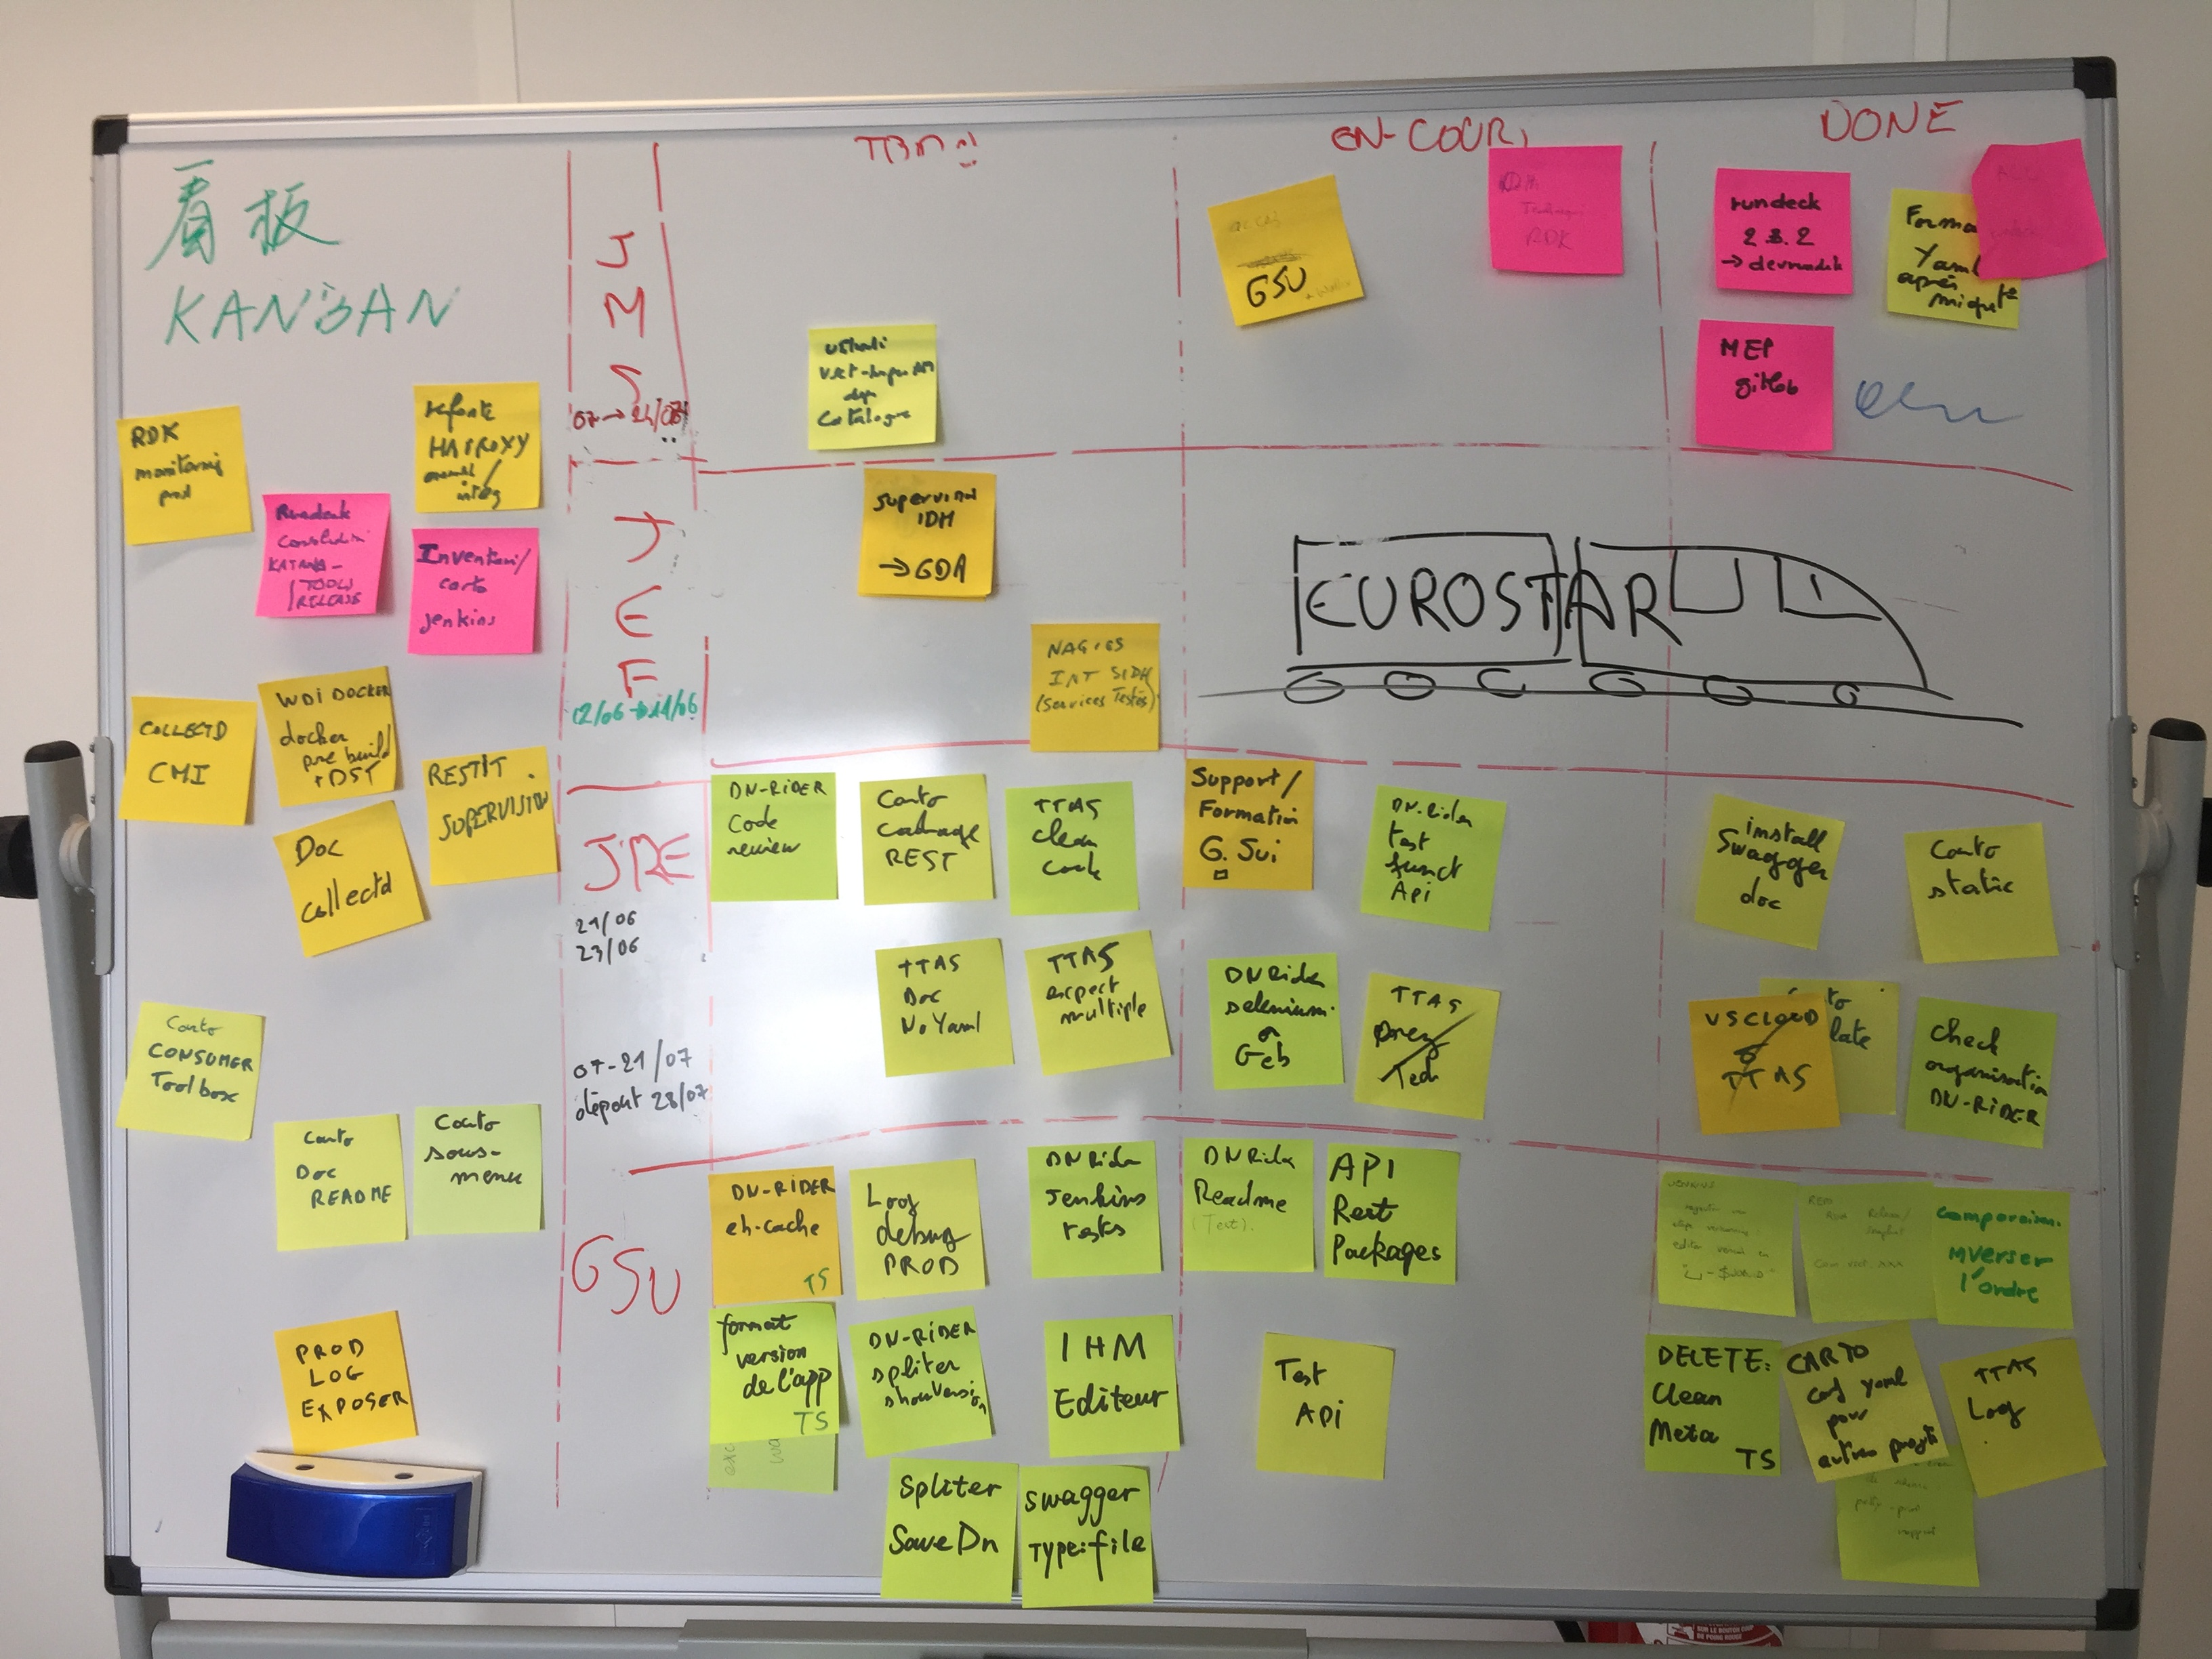
\includegraphics[width=0.8\textwidth]{kanban}
\caption{Kanban}
\end{figure}

\clearpage

\section{Application}
\paragraph{présentation: IHM, Api REST(swagger), Continus Delivery(git, test unitaire, pipeline->deploiement auto)}
\paragraph{arch}
\subparagraph{choix de techno: groovy, grails(référent compétent), bootstrap, jquery(justificatif)/backlog}
\subparagraph{archi appli: modèle MVC, lien vers Nexus}

\clearpage

\section{Etat fin de stage}
\paragraph{1 application opérationnelle sur serveur PROD}
\paragraph{démo au sein de l’équipe (FUTUR démo global)}
\paragraph{bilan objectif de l’appli}

\clearpage
